\documentclass[a4paper,10pt]{article}
\usepackage[utf8]{inputenc}
\usepackage[brazilian]{babel}
\usepackage{graphicx}        % standard LaTeX graphics tool
\usepackage{color,enumerate}
\usepackage{subfigure}
\usepackage{tikz}
\usepackage{fullpage,amsmath,amssymb}
\title{2022-2: Lista de exercícios 01}
\author{Ronaldo de Freitas Zampolo}

\begin{document}
Universidade Federal do Pará

Instituto de Tecnologia

Faculdade de Engenharia da Computação e Telecomunicações

EC01045 - Processamento digital de sinais

Prof. Ronaldo de Freitas Zampolo

\begin{center} \textsc{2022-2: Lista de exercícios 01} \end{center}

%\maketitle
\begin{enumerate}
	\item Seja um sistema discreto LI (linear e invariante), cuja resposta ao impulso é 
		\begin{equation*}
			h[n] = \delta[n] + \delta[n-1]
		\end{equation*}
		\begin{enumerate}
			\item Determine a resposta em frequência deste sistema $H(e^{j\omega})$, se possível.
			\item Calcule a função de transferência $H(z)$.
			\item Esboce o diagrama de pólos e zeros, indicando também a região de convergência.
			\item Que tipo de sistema é esse? Marque a resposta correta e justifique sua resposta.
				\begin{enumerate}
					\item Passa-baixas
					\item Passa-altas
					\item Passa-banda
					\item Rejeita-banda
				\end{enumerate}
			\item A resposta ao impulso desse sistema é do tipo:
				\begin{enumerate}
					\item FIR
					\item IIR, à direita
					\item IIR, à esquerda
					\item IIR, bilateral
				\end{enumerate}
				Marque e justifique sua resposta.
			\item O sistema é estável? Justifique sua resposta usando a região de convergência de $H(z)$.
			\item Ache a equação de diferenças para o sistema.
		\end{enumerate}
	\item Um sistema LI tem resposta ao impulso dada pelo gráfico
		\begin{figure*}[h]
			\centering
			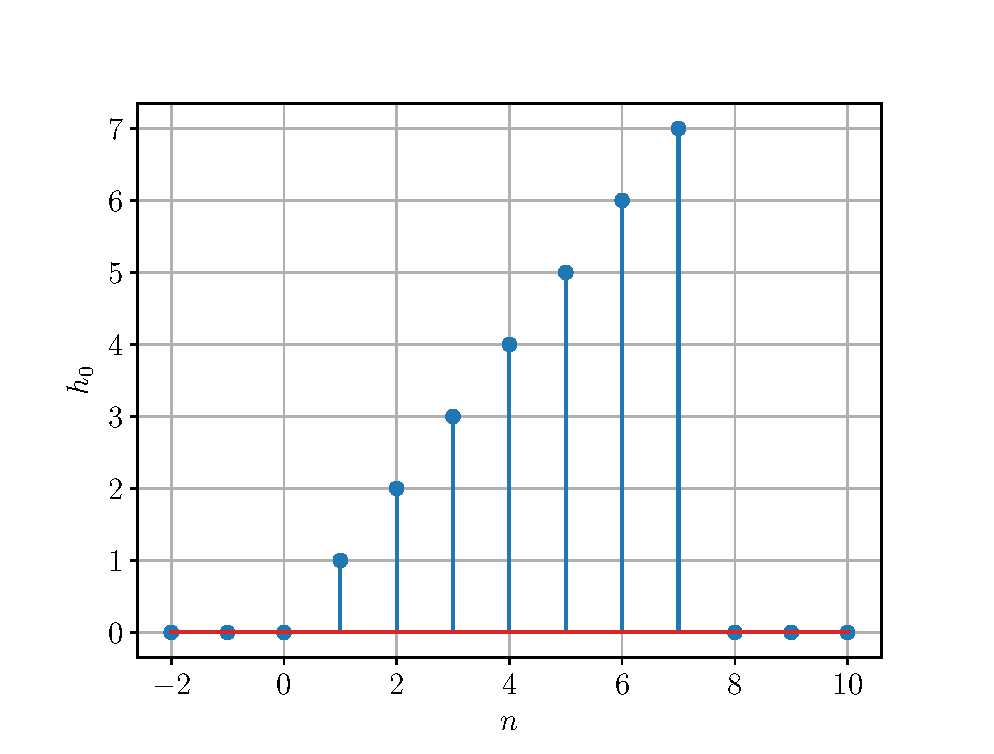
\includegraphics[width=0.65\textwidth]{figs/h0}
			\label{fig:h0}
			\caption{Resposta ao impulso.}
		\end{figure*}
		\begin{enumerate}
			\item Qual a função de transferência $H_0(z)$ do sistema? Calcule pólos e zeros, e indique-os no plano complexo Z.
			\item Suponha que $H_1(z) = H_0(-z)$. Determine os pólos e zeros de $H_1(z)$, indicando-os no plano complexo Z.
			\item Determine $h_1[n]$.
	        \end{enumerate}
	% questão 3.22 do livro-texto
	\item Um sistema LI causal tem função de sistema
		\begin{equation*}
			H(z) = \frac{1-4z^{-1}}{1+0,5z^{-1}}.
		\end{equation*}
		A entrada desse sistema é
		\begin{equation*}
			x[n] = u[n] + 2\cos\left (\frac{\pi}{2}n\right )\qquad -\infty< n < \infty
		\end{equation*}
		Determine a saída $y[n]$ para um $n$ grande e positivo; isto é, encontre uma expressão para $y[n]$ que seja assintoticamente correta quando $n$ se torna grande. Naturalmente, uma possível abordagem é encontrar uma expressão para $y[n]$ que seja válida para todo $n$, mas há um modo mais fácil (que você deve usar).
	
	% questão 3.30 do livro-texto
	\item Um sistema LI causal tem função de sistema
		\begin{equation*}
			H(z) = \frac{1-z^{-1}}{1-0,25z^{-2}} = \frac{1-z^{-1}}{(1-0,5z^{-1})(1+0,5z^{-1})}
		\end{equation*}
		\begin{enumerate}
			\item Determine a saída do sistema quando a entrada é $x[n]=u[n]$.
			\item Determine a entrada $x[n]$, de modo que a saída correspondente do sistema seja $y[n]=\delta[n] - \delta[n-1]$.
			\item Determine a saída $y[n]$ quando a entrada $x[n] = \cos(0,5\pi n)$ para $-\infty < n< \infty$.
		\end{enumerate}

	\item  Considere um sistema LI causal, cuja relação entre entrada e saída é representada pela equação de diferenças
		\begin{equation*}
			y[n] - 2 y[n-1] = x[n]
		\end{equation*}
		\begin{enumerate}
			\item Determine a resposta do sistema ao impulso e ao degrau unitário.
			\item Calcule a função de transferência do sistema $H(z)$.
			\item Encontre os pólos e zeros.
			\item Avalie a estabilidade do sistema, justificando sua resposta.
		\end{enumerate}
	\item O sistema LI causal da questão anterior, representado aqui pela resposta ao impulso $h_0[n]$, é utilizado em um novo arranjo (ver figura a seguir), onde $\alpha$ é um número real maior que zero e $w[n]=x[n]-\alpha y[n-1]$.
		\begin{figure*}[h]
			\centering
			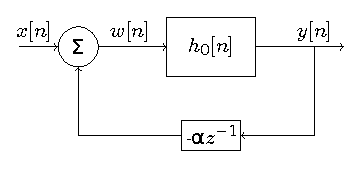
\includegraphics[width=0.45\textwidth]{figs/arranjo}
			\label{fig:arranjo}
			\caption{Arranjo com realimentação.}
		\end{figure*}

		Para $\alpha = 0,5$ e $\alpha = 1,5$:
		\begin{enumerate}
			\item Determine a resposta do sistema ao impulso e ao degrau unitário.
			\item Calcule a função de transferência do sistema $H(z)=Y(z)/X(z)$.
			\item Encontre os pólos e zeros.
			\item Avalie a estabilidade do sistema, justificando sua resposta.
		\end{enumerate}

	%	\begin{enumerate}Questão envolvendo transformada Z inversa (elaborada)
	%\item Mais uma questão: fourier e z, equ. de diferenças, resposta por convolução e transformada z (transformada z inversa)
	%\item Resposta ao impulso por resolução de equação homogênea e comparação com resposta obtida por transformada z inversa
\end{enumerate}
\end{document}
